\documentclass[11pt]{article}
\usepackage[english]{babel}
\usepackage{minted}
\usepackage{amsmath}
\usepackage{amsthm}
\usepackage{graphicx}
\usepackage{subcaption}
\usepackage{booktabs}
\usepackage[left=25mm, top=25mm, bottom=30mm, right=25mm]{geometry}
\usepackage[colorlinks=true, linkcolor=blue, urlcolor=cyan]{hyperref}

\title{COL380 Assignment 1}
\author{Sayam Sethi}
\date{January 2022}

\begin{document}

\maketitle

\tableofcontents

\section{Implementation}
The following steps give an idea of the implementation and design choices:
\begin{enumerate}
	\item Merge sort was used for \texttt{SequentialSort}.
	\item \texttt{SequentialSort} was called if $n / p < p$ since $p^2$ pseudo splitters cannot be selected in this case.
	\item The first $n\mod p$ buckets contain $n/p + 1$ elements and the remaining buckets contain $n/p$ elements.
	\item $A_i$'s are not constructed explicitly in the code and $R$ is generated directly from $A$.
	\item $R$ is sorted and the array $S$ is considered implicitly as the elements of $R$ at suitable indices.
	\item Using tasks, the array $A$ was split into almost equal $p$ partitions and a task was scheduled for each partition. The bin for each element was computed (using binary search) and the number of elements in each bin for each thread.
	\item The counts for each bin across different threads were summed up.
	\item Using tasks, $p$ arrays $B_i$'s were created for each bin of length computed via the counts in the previous step. Each task copied corresponding elements from $A$.
	\item Prefix sum of counts was computed.
	\item Using tasks, $B_i$'s were copied back to $A$ at the correct locations and the corresponding subset was sorted by \texttt{SequentialSort} or \texttt{ParallelSort} depending on the size.
\end{enumerate}

\section{Time and Space Complexity}

\subsection{Time Complexity}
The average case time complexity of \texttt{ParallelSort} is given as:
\begin{equation}
	\begin{split}
		&O(p^2) + O(p^2 \log{p}) + O\left(n + \frac{n \log{p}}{t}\right) + O(p\cdot t) + O\left(\frac{p\cdot n}{t}\right) + O\left(\frac{p\cdot (n/p + n/p\log(n/p))}{t}\right)\\
		=&O\left(p^2(1 + \log{p}) + n + pt + \frac{(p + 1)n + n\log{n}}{t}\right)
	\end{split}
\end{equation}
The assumption made in the above analysis is that the bins are almost euqally split such that no bin has a size larger than the threshold. Also, $t$ above is the number of threads.

\subsection{Space Complexity}
The average case space complexity is given as:
\begin{equation}
	O(p^2) + O(p\cdot t) + O(n) + O(p) + O(n) + O(n) = O(p^2 + pt + n)
\end{equation}
Again, the same assumption is made that \texttt{SequentialSort} is called for each bin and thus the space complexity of the function call is $O(n)$ and the remaining space is used for the arrays declared in the \texttt{ParallelSort} function.

\section{Parallelism and Scalability}
From the time complexity, it is clear that the entire function cannot be parallelised and an $O(n)$ term remains outside the parallel execution. Additionally, the parallel execution involves an $O(pn)$ term (when updating $B_i$'s) which isn't truly parallel. Although, the same loop could have been converted to an $O(n)$ non-parallel loop, however, the same would involve significant cache misses due to the random nature of the bins of consecutive elements.\par
Following are the plots for different values of $n$ and $p$ and comments for the same are followed:

\subsection{Graphs}
\begin{figure}[H]
	\begin{center}
		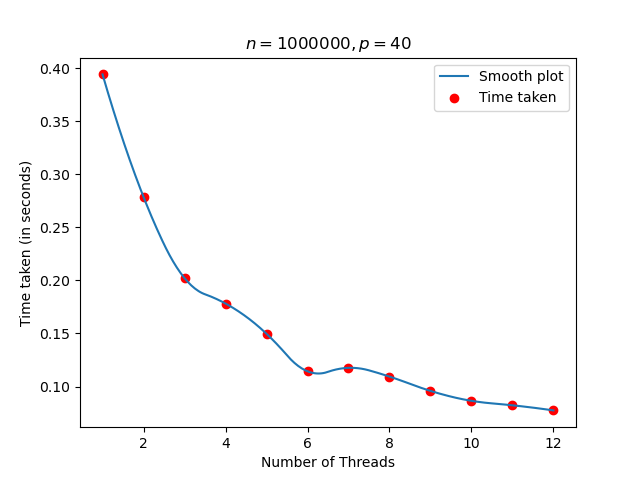
\includegraphics[width=0.5\textwidth]{outputs/1e6_40_t12.png}
	\end{center}
	\caption{$n = 10^6, p = 40$}
	\label{fig:1e6_40}
\end{figure}
The scalability for this case is $5.09\times$ for $12$ cores, from $394.356ms$ to $77.4758ms$. There is linear decrease until $3$ cores and the absolute value of the slope decreases after that. The value of slope decreases even further from $7$ cores (and remains almost constant from $6$ to $7$ cores).

\begin{figure}[H]
	\begin{center}
		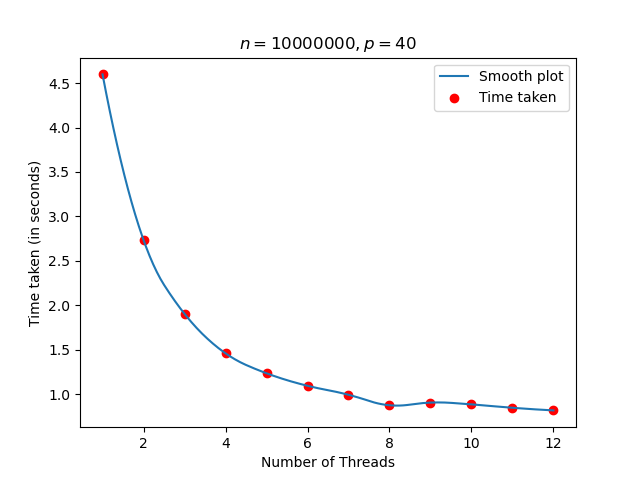
\includegraphics[width=0.5\textwidth]{outputs/1e7_40_t12.png}
	\end{center}
	\caption{$n = 10^7, p = 40$}
	\label{fig:1e7_40}
\end{figure}
The scalability for this is $5.63\times$ for $12$ cores, from $4598.39ms$ to $816.751ms$. The curve follows an asymptotic pattern and the running time almost saturates by $8$ cores. The scalability upto $8$ cores is $5.25\times$. The constancy is partly due to the fact that when scheduling tasks, the division cannot be done equally across all threads and some threads work on fewer loops than the other threads.

\begin{figure}[H]
	\begin{center}
		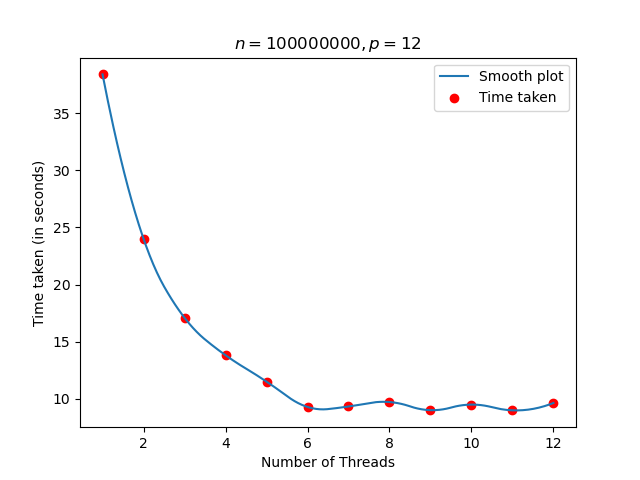
\includegraphics[width=0.5\textwidth]{outputs/1e8_12_t12.png}
	\end{center}
	\caption{$n = 10^8, p = 12$}
	\label{fig:1e8_12}
\end{figure}
The maximum scalability for this is $4.27\times$ for $11$ cores, from $38.389s$ to $8.99421s$. This is much lesser than the scalability in the previous parts. This is due to the fact that the number of bins is fewer and thus the probability of equal division of work reduces. The running time saturates by $6$ cores and the scalability then is $4.13$. Additionally, the fluctuations in running time for $8, 10, 12$ threads is due to the scheduling scenario where some threads need to perform comparatively more tasks. This increases the execution time.

\begin{figure}[H]
	\begin{center}
		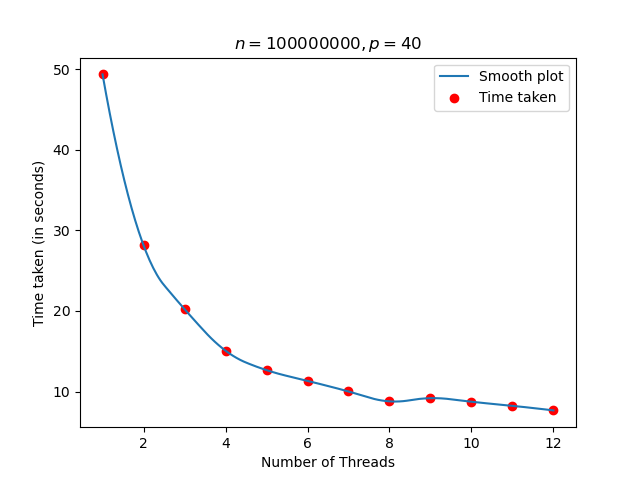
\includegraphics[width=0.5\textwidth]{outputs/1e8_40_t12.png}
	\end{center}
	\caption{$n = 10^8, p = 40$}
	\label{fig:1e8_40}
\end{figure}
The scalability is $6.43\times$ for $12$ cores, from $49.3318s$ to $7.67387s$. This situation doesn't have the limitation of reaching saturation like the previous graph. Therefore, the speedup slows down towards $12$ cores but there is still a linear improvement from $9$ to $12$ cores.

\begin{figure}[H]
	\begin{center}
		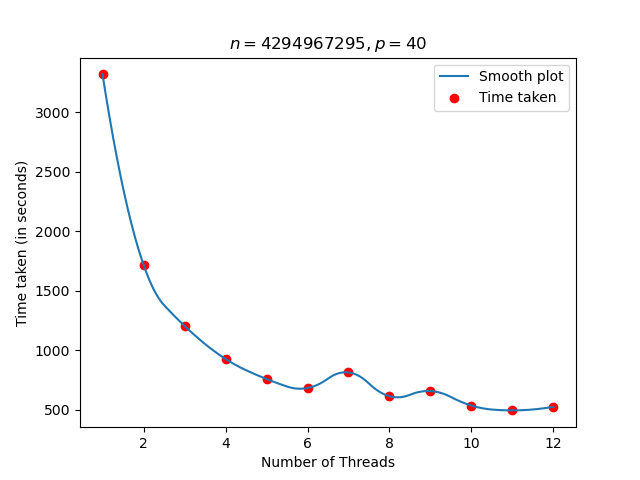
\includegraphics[width=0.5\textwidth]{outputs/4294967295_40_t12.png}
	\end{center}
	\caption{$n = 2^{32} - 1, p = 40$}
	\label{fig:4294967295_40}
\end{figure}
The maximum scalability achieved is $6.70\times$ for $11$ cores, from $55.3285$ minutes to $8.2608$ minutes. There is significant fluctuation towards large number of cores, however, the general trend is that the running time is significantly reducing even at $12$ cores. The same isn't visible in the graph due to the large amount of time taken for fewer number of cores.

\subsection{Conclusion}
The maximum speedup obtained in the entire analysis was $6.70\times$. The best efficiency of the parallelisation was $0.56$. The speed-up would have been better if the analysis could have been performed upto $24$ cores however, due to limited resources on HPC, the same could not be done. Overall, every possible loop in the function \texttt{ParallelSort} was parallelised and any further optimisation would be micro-optimisations, especially in memory allocation.\par
\textbf{Note:} In the entire discussion above, the number of cores is the same as the number of threads.

\end{document}
